\begin{figure}
  \caption{Dependence of Social Learning ($\langle s \rangle$) on environmental
  variability $u$ for several values of low payoff $\pi_{low}$ and steps per
  round, $M$. $\langle s \rangle$ decreases monotonically for $\pi_{low} = 0.1, 0.5$,
but noise dominates the results for $\pi_{low}=0.8$. When $\pi_{low} = 0.5$, 
the sigmoid is not as sharp as for $\pi_{low}=0.1$, meaning that social learning
is reduced for smaller $u$ and increased for larger $u$.}
  \label{fig:results}
  \centering
  \begin{subfigure}[t]{0.33\textwidth}
    \centering
  \caption{$B = 2$, $M=1,2,4$ (50 TRIALS)}
    \includegraphics[width=\textwidth]{
      {Figures/SL_over_u_lowpayoff=0.1_nbehaviors=2.pdf}
    }
    \centering
    \includegraphics[width=\textwidth]{
      {Figures/SL_over_u_lowpayoff=0.5_nbehaviors=2.pdf}
    }
    \includegraphics[width=\textwidth]{
      {Figures/SL_over_u_lowpayoff=0.8_nbehaviors=2.pdf}
    }
  \end{subfigure}%
  \begin{subfigure}[t]{0.33\textwidth}
    \centering
    \caption{$B = 4$, $M=2,4,8$ (20 TRIALS)}
    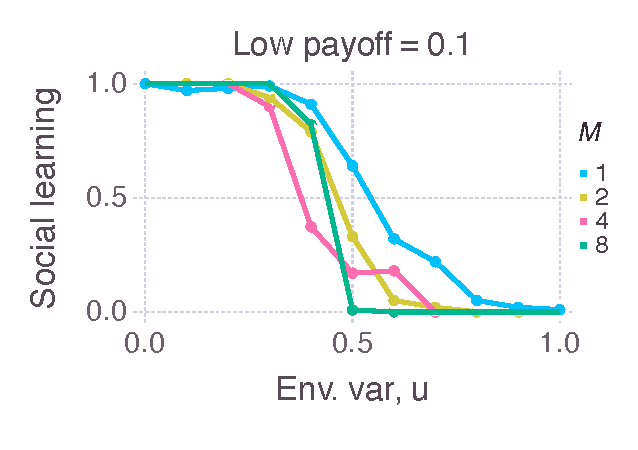
\includegraphics[width=\textwidth]{
      {Figures/SL_over_u_lowpayoff=0.1_nbehaviors=4.pdf}
    } \\
    \centering
    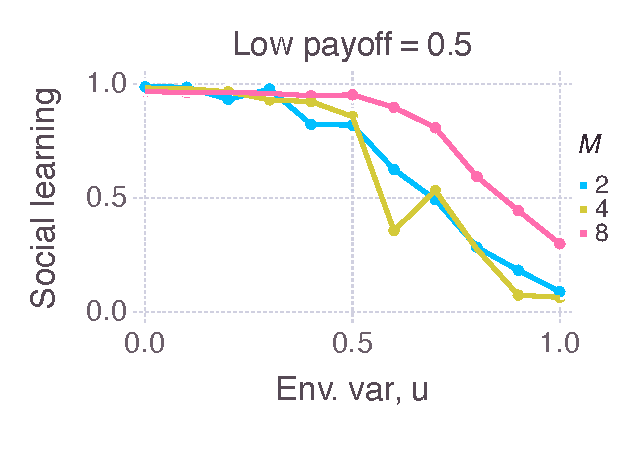
\includegraphics[width=\textwidth]{
      {Figures/SL_over_u_lowpayoff=0.5_nbehaviors=4.pdf}
    } \\
    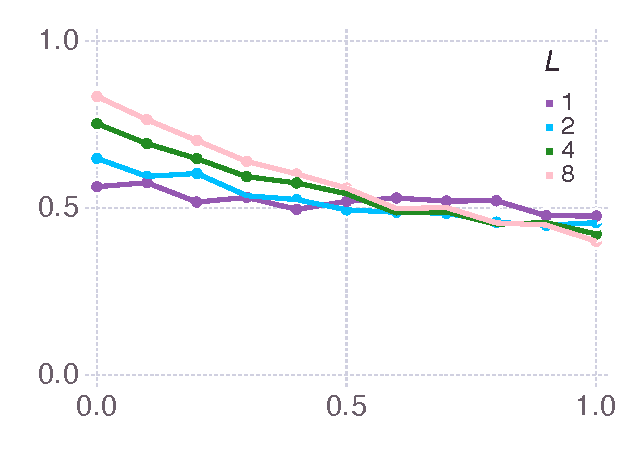
\includegraphics[width=\textwidth]{
      {Figures/SL_over_u_lowpayoff=0.8_nbehaviors=4.pdf}
    }
  \end{subfigure}
  \begin{subfigure}[t]{0.33\textwidth}
    \centering
    \caption{$B = 10$, $M=5,10,20$ (20 TRIALS)}
    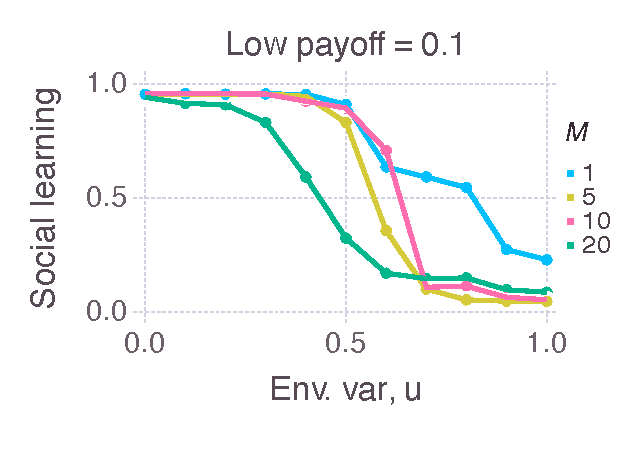
\includegraphics[width=\textwidth]{
      {Figures/SL_over_u_lowpayoff=0.1_nbehaviors=10.pdf}
    } \\
    \centering
    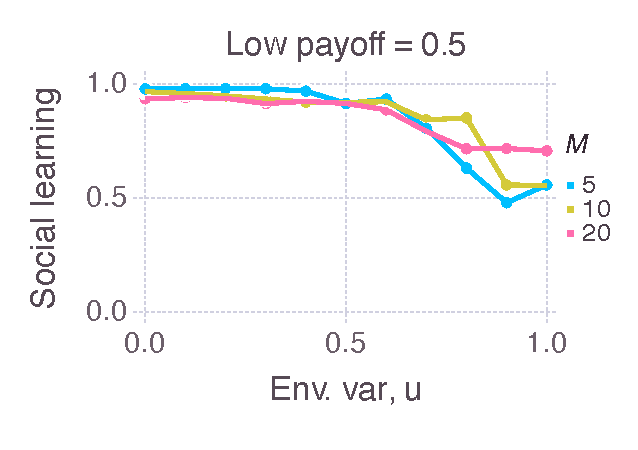
\includegraphics[width=\textwidth]{
      {Figures/SL_over_u_lowpayoff=0.5_nbehaviors=10.pdf}
    } \\
    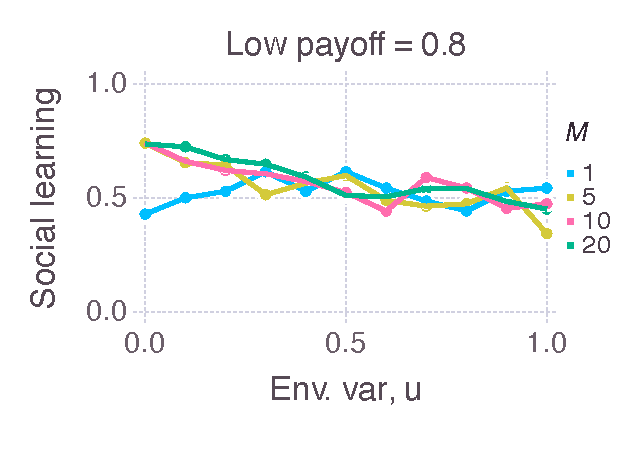
\includegraphics[width=\textwidth]{
      {Figures/SL_over_u_lowpayoff=0.8_nbehaviors=10.pdf}
    }
  \end{subfigure}
  
  
\end{figure}


% \begin{figure}
%   \centering
%   \begin{subfigure}[t]{0.3\textwidth}
%     \centering
%     \textbf{A}%
%     \includegraphics[width=\textwidth]{
%       {Figures/SL_over_u_lowpayoff=0.1_nbehaviors=2.pdf}
%     }
%   % \caption{}
%   % \label{fig:results_pilow_0p1}
%   \end{subfigure}%
%   \begin{subfigure}[t]{0.3\textwidth}
%     \centering
%     \includegraphics[width=\textwidth]{
%       {Figures/SL_over_u_lowpayoff=0.5_nbehaviors=2.pdf}
%     }
%   % \caption{}
%   % \label{fig:}
%   \end{subfigure}%
%   \begin{subfigure}[t]{0.3\textwidth}
%     \centering
%     \includegraphics[width=\textwidth]{
%       {Figures/SL_over_u_lowpayoff=0.8_nbehaviors=2.pdf}
%     }
%   % \caption{}
%   % \label{fig:}
%   \end{subfigure}
  
%   \caption{Dependence of Social Learning ($\langle s \rangle$) on environmental
%   variability $u$ for several values of low payoff $\pi_{low}$ and steps per
%   round, $M$. $\langle s \rangle$ decreases monotonically for $\pi_{low} = 0.1, 0.5$,
% but noise dominates the results for $\pi_{low}=0.8$. When $\pi_{low} = 0.5$, 
% the sigmoid is not as sharp as for $\pi_{low}=0.1$, meaning that social learning
% is reduced for smaller $u$ and increased for larger $u$.}
%   \label{fig:results}
% \end{figure}
